\documentclass{beamer}
\usetheme{Boadilla}
%\usetheme{Malmoe}
%\usetheme{Antibes}
%\usetheme{Warsaw}

\usepackage[utf8]{inputenc}
\usepackage{wasysym}
\usepackage{multirow} %para mesclar linhas
\usepackage{booktabs} %para definir tamanho de linha na tabela
\usepackage{ragged2e} %para o comando \justifying que deixa o texto justificado
\usepackage{pslatex}
\usepackage{listings}
\usepackage{xcolor}

\definecolor{codegreen}{rgb}{0,0.6,0}
\definecolor{codegray}{rgb}{0.5,0.5,0.5}
\definecolor{codeorange}{rgb}{1,0.49,0}
\definecolor{backcolour}{rgb}{0.95,0.95,0.96}

\lstdefinestyle{mystyle}{
    backgroundcolor=\color{backcolour},   
    commentstyle=\color{codegray},
    keywordstyle=\color{codeorange},
    numberstyle=\tiny\color{codegray},
    stringstyle=\color{codegreen},
    basicstyle=\ttfamily\footnotesize,
    breakatwhitespace=false,         
    breaklines=true,                 
    captionpos=b,                    
    keepspaces=true,                 
    numbers=left,                    
    numbersep=5pt,                  
    showspaces=false,                
    showstringspaces=false,
    showtabs=false,                  
    tabsize=2,
    xleftmargin=10pt,
}

\lstset{style=mystyle}

\title{Tópicos de programação não síncrona}
\author{Evandro Paulo Folletto}
\institute[Volpi]{Volpi.tech}
\date{2023}

\AtBeginSection[]{  %Comando para aparecer o sumário na frente de cada seção nova
	\tableofcontents[currentsection]
	\newpage
}

\AtBeginSubsection[]{  %Comando para aparecer o sumário na frente de cada subseção nova
	\tableofcontents[currentsubsection]
	\newpage
}

\begin{document}

	\begin{frame}
	 \titlepage
	\end{frame}

	\tableofcontents
	\newpage

	\section{Concorrência x Paralelismo}
 	\textbf{Concorrência:} capacidade de executar sequencialmente um conjunto de tarefas independentes. \\
	\textbf{Paralelismo:} execução de mais de uma tarefa por vez (de forma simultânea), a depender da quantidade de núcleos (cores) do processador. Quanto mais núcleos, mais tarefas paralelas podem ser executadas.
	\begin{figure}
 	 \centering
 	 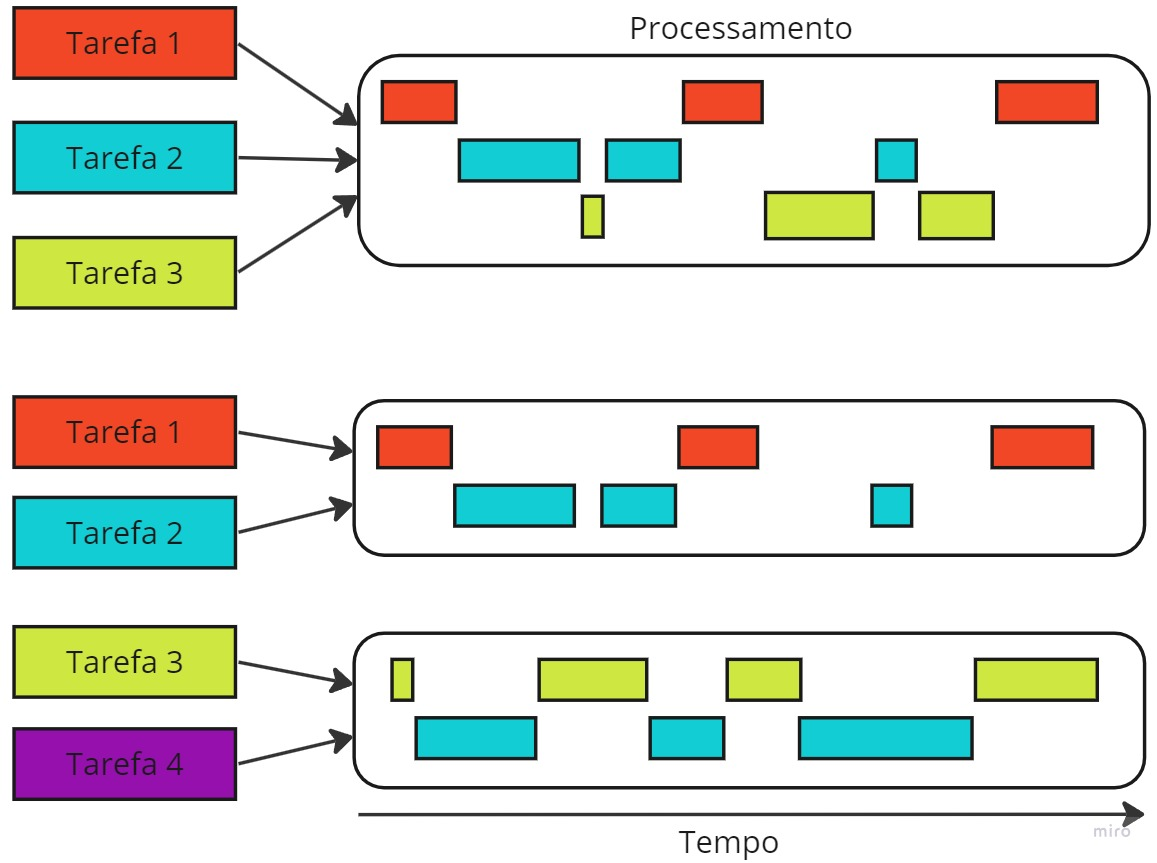
\includegraphics[scale=0.2]{figuras/concorrencia_paralelismo.jpg}
	\end{figure}
	\newpage

	\section{Estilo de programação sequencial x paralelo}
 	\textbf{Sequencial:} as instruções são executadas uma após a outra, em uma ordem predefinida. Cada instrução é executada completamente antes que a próxima seja iniciada, de forma linear. \\
	\textbf{Paralelismo:} as instruções são executadas simultaneamente em múltiplos processadores ou núcleos de processamento, permitindo que várias instruções sejam processadas simultaneamente.
	\begin{figure}
 	 \centering
 	 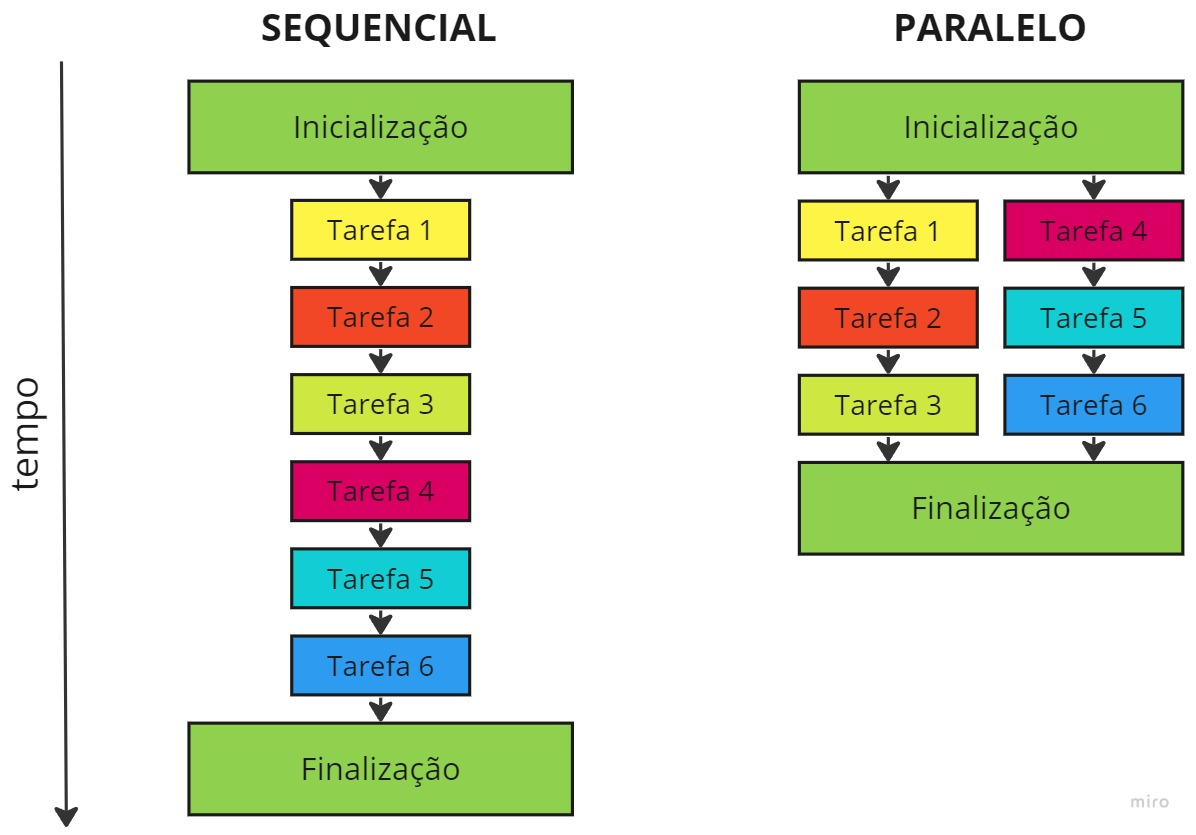
\includegraphics[scale=0.2]{figuras/sequencial_paralelo.jpg}
	\end{figure}
	\newpage

%	Abaixo é mostrado um exemplo de código sequencial:
%	\begin{lstlisting}[language=Python, caption={Código sequencial.}, mathescape=true, breaklines=true, basicstyle=\tiny]
%		from time import sleep
%
%		def tarefa1():
%    		sleep(5)
%	   	 print('estou dentro da tarefa1')
%
%		def tarefa2():
%	    	sleep(5)
%    		print('estou dentro da tarefa2')
%
%		def tarefa3():
%	    	sleep(5)
%    		print('estou dentro da tarefa3')
%
%		tarefa1()
%		tarefa2()
%		tarefa3()
%	\end{lstlisting}
%	\newpage

%	Abaixo é mostrado um exemplo de código paralelo, utilizando a biblioteca 'threading':
%	\begin{lstlisting}[language=Python, caption={Código paralelo.}, mathescape=true, breaklines=true, basicstyle=\tiny]
%		from time import sleep
%		import threading
%
%		def tarefa1():
%    		sleep(5)
%		    print('estou dentro da tarefa1')
%
%		def tarefa2():
%    		sleep(5)
%		    print('estou dentro da tarefa2')
%
%		def tarefa3():
%    		sleep(5)
%		    print('estou dentro da tarefa3')
%
%		threading.Thread(target=tarefa1, name=tarefa1).start()
%		threading.Thread(target=tarefa2, name=tarefa2).start()
%		threading.Thread(target=tarefa3, name=tarefa3).start()
%		
%		print('estou neste ponto!')
%	\end{lstlisting}
%	\newpage

	\section{Multithreading x Multiprocessamento}
	A utilização dos conceitos de multithreading e multiprocessamento para computação paralela e consequente ganho de desempenho é bastante difundida. Mas em Python existem particularidades: \\ 
	\textbf{Multithreading:} útil para operações de E/S ou tarefas vinculadas à rede, como a execução de scripts, por exemplo, no caso de web scraping. As \textit{threads} não podem alcançar o paralelismo completo aproveitando vários núcleos de CPU devido a restrições GIL em Python. \\
 	\textbf{GIL (Global Lock Interpreter):} só deixa uma thread por vez executar, isso acontece pois o python não é \textit{Thread Safe} o que significa que diferentes threads podem ter acesso a memória de forma indevida e causar quebras no programa. Isso pode resultar em pior performance. \\
	$\rightarrow$ Para utilizar Multithreading (pacote python): import threading. \\
 	\textbf{Multiprocessamento:} é uma escolha adequada caso as tarefas sejam extensas da CPU e não tenham nenhuma operação de E/S ou interações do usuário. Exemplos: algoritmos de \textit{machine learning} e \textit{deep learning}. \\
	$\rightarrow$ Para utilizar Multiprocessamento (pacote python): import multiprocessing. \\
	\newpage

	\alert{\textbf{Exemplos:}} \\

	\begin{itemize}
		\item Exemplo 1 \\
			\begin{itemize}
				\item ./exemplo\textunderscore 1/main\textunderscore A.py: exemplo utilizando sincronicidade \\
				\item ./exemplo\textunderscore 1/main\textunderscore B.py: exemplo utilizando multithreading \\
				\item ./exemplo\textunderscore 1/main\textunderscore B2.py: exemplo utilizando multithreading e podendo receber uma lista de tarefas \\				
				\item ./exemplo\textunderscore 1/main\textunderscore C.py: exemplo utilizando multiprocessamento \\
		 	\end{itemize}
		\item Exemplo 2 \\
			\begin{itemize}
				\item ./exemplo\textunderscore 2/main\textunderscore A.py: exemplo utilizando sincronicidade \\
				\item ./exemplo\textunderscore 2/main\textunderscore B.py: exemplo utilizando multithreading \\			
				\item ./exemplo\textunderscore 2/main\textunderscore C.py: exemplo utilizando multiprocessamento \\
				\item ./exemplo\textunderscore 2/main\textunderscore D.py: exemplo utilizando multiprocessamento e podendo receber uma lista de tarefas \\				
		 	\end{itemize}		 	
 	\end{itemize}
	\newpage

	\section{Filas de tarefas com Celery}
	Celery é uma ferramenta que possibilita a criação de filas de tarefas (\textit{task queues}), que é um mecanismo que permite distribuir tais tarefas entre \textit{threads} ou processos diferentes. Ou seja, a execução dessas tarefas ocorre de forma independente do nosso programa e, dessa forma, podemos mandar o computador executar uma operação custosa pelo Celery em, por exemplo, um banco de dados, enquanto o nosso programa prossegue com o roteiro. \\
	$\rightarrow$ Instalação Celery: pip install celery \\
	$\rightarrow$ Iniciar o Celery: celery -A $<$nome\textunderscore arquivo$>$ worker -l info --pool=solo	
	\textbf{Broker:} o Celery precisa de pelo menos um mediador (\textit{broker}) onde informações sobre as tarefas serão enfileiradas. Exemplos: RabbitMQ, \underline{Redis}, Amazon SQS e Zookeeper. \\
	$\rightarrow$ Instalação Redis: pip install redis \\
	$\rightarrow$ Iniciar o Redis no docker: docker run -d -p 6379:6379 redis \\
	\textbf{Flower:} ferramenta web para monitorar e administrar clusters Celery. \\
	$\rightarrow$ Instalação Flower: pip install flower \\
	$\rightarrow$ Iniciar o Flower: celery -A $<$nome\textunderscore arquivo$>$ flower --address=127.0.0.6 --port=5566
	\newpage

	\alert{\textbf{Exemplos:}} \\

 	\begin{itemize}
   		\item ./exemplo\textunderscore 3/A: \\
	 		\begin{itemize}
				\item main.py: exemplo sem utilização do Celery. \\
				\item tasks.py: exemplo sem utilização do Celery. \\
		 	\end{itemize}
   		\item ./exemplo\textunderscore 3/B: \\
	 		\begin{itemize}
				\item main.py: exemplo com utilização do Celery. \\
				\item tasks.py: exemplo com utilização do Celery. \\
		 	\end{itemize}
   		\item ./exemplo\textunderscore 3/C: \\
	 		\begin{itemize}
				\item main.py: exemplo utilizando método Chain. \\
				\item tasks.py: exemplo utilizando método Chain. \\
			 \end{itemize}  					
	\end{itemize}

	\newpage

	\section{Programação assíncrona com AsyncIO e Async/Await}
	Introduzida em 2012, a biblioteca \textit{asyncio} fornece à linguagem recursos para a criação de código concorrente sem precisar recorrer ao uso de múltiplas \textit{threadings}, utilizando \textit{event loops} em seu lugar. O \textit{asyncio} é hoje o módulo padrão em Python para atingir concorrência através de uma única \textit{thread}. \\
	$\rightarrow$ Instalação AsyncIO: pip install asyncio \\
	A sintaxe do Python utiliza duas palavras reservadas: \\
 	\textbf{async:} indica que uma função deve ser executada de forma assíncrona. \\
 	\textbf{await:} significa que a corrotina será paralisada naquele ponto aguardando um resultado futuro. \\
 	Em outras palavras, o controle de execução será dado à outra corrotina e só será retomado quando o resultado ficar pronto.

	\alert{\textbf{Exemplos:}} \\
	\begin{itemize}
		\item ./exemplo\textunderscore 4/main\textunderscore A.py: exemplo utilizando sincronidade \\
		\item ./exemplo\textunderscore 4/main\textunderscore B.py: exemplo utilizando asyncio \\
		\item ./exemplo\textunderscore 4/main\textunderscore C.py: exemplo utilizando asyncio, mas reescrito para receber uma lista de tarefas\\
 	\end{itemize}
	\newpage

	\section{Solicitações HTTP assíncronas: aiohttp}
	A biblioteca aiohttp é utilizada para fazer solicitações HTTP assíncronas, que é um dos casos de uso mais comuns do código sem bloqueio. \\
	$\rightarrow$ Instalação aiohttp: pip install aiohttp \\
	Exemplo documentação (\url{https://pypi.org/project/aiohttp}):
	\begin{lstlisting}[language=Python, mathescape=true, breaklines=true, basicstyle=\tiny]
	import aiohttp
	import asyncio

	async def main():

    	async with aiohttp.ClientSession() as session:
        	async with session.get('http://python.org') as response:

            	print("Status:", response.status)
            	print("Content-type:", response.headers['content-type'])

            	html = await response.text()
            	print("Body:", html[:15], "...")

	asyncio.run(main())
	\end{lstlisting}

	\alert{\textbf{Exemplos:}} \\
	\begin{itemize}
		\item ./exemplo\textunderscore 5/main\textunderscore A.py: exemplo utilizando solicitações síncronas \\
		\item ./exemplo\textunderscore 5/main\textunderscore B.py: exemplo utilizando aiohttp \\
		\item ./exemplo\textunderscore 5/main\textunderscore C.py: exemplo utilizando aiohttp e tarefas do asyncio \\
 	\end{itemize}
	\newpage
	
\end{document}